%% model_theory.tex
%% 世界经济形成的智能体模拟模型：理论依据、设计思想与规则
%% ECON0302G 课程研究报告

\documentclass[12pt, a4paper]{article}

\usepackage[UTF8]{ctex}
\usepackage{amsmath, amssymb, amsthm}
\usepackage{geometry}
\usepackage{booktabs}
\usepackage{array}
\usepackage{hyperref}
\usepackage{setspace}
\usepackage{enumitem}
\usepackage{caption}
\usepackage{graphicx}
\usepackage{subcaption}
\usepackage{float}
\usepackage{xcolor}
\usepackage{tabularx}
\graphicspath{{./discovery/}}

\geometry{top=2.5cm, bottom=2.5cm, left=3cm, right=3cm}
\onehalfspacing

\title{\textbf{世界经济格局形成的智能体模拟模型}\\
       \large 理论依据、设计思想与量化规则}
\author{ECON0302G · 世界经济导论}
\date{\today}

\begin{document}

\maketitle
\tableofcontents
\newpage

% ──────────────────────────────────────────────────────────────────
\section{研究问题与建模动机}
% ──────────────────────────────────────────────────────────────────

本模型旨在检验世界经济格局形成中\textbf{地理初始条件}、\textbf{战略选择}与\textbf{历史偶然性}三类因素的相对贡献。核心研究问题为：在给定相同历史制度和技术起点的前提下，初始地理禀赋能在多大程度上决定1000--1850年间各文明的经济分化？如果中国延续郑和式的航海扩张政策，或英国缺乏可通航水道旁的煤炭，均衡结果将如何改变？

为回答上述反事实问题，本文构建了一个\textbf{文明级多智能体仿真系统}（Multi-Agent Historical Simulation），结合文明策略游戏的叙事框架与强化学习方法，在受控实验环境中多次运行历史路径，形成结果分布，进而分解各因素的方差贡献。

% ──────────────────────────────────────────────────────────────────
\section{模型整体架构}
% ──────────────────────────────────────────────────────────────────

模型由三层结构组成：

\begin{enumerate}[label=\textbf{\arabic*.}]
    \item \textbf{状态层（State Layer）}：每个智能体（文明/国家）维护一组连续状态变量，包括人口、GDP、资本存量、技术水平向量、领土规模及贸易开放度。
    \item \textbf{决策层（Decision Layer）}：每回合每个文明由绑定的策略代理（rule-based 或 Q-learning）选择离散动作，映射为技术投资偏好、贸易政策与扩张力度三个维度。
    \item \textbf{动态层（Dynamics Layer）}：经济引擎按照柯布—道格拉斯生产函数、Logistic人口方程、资本积累方程及贸易收益公式更新全部文明状态；历史随机事件作为外生扰动项施加于若干文明。
\end{enumerate}

时间轴被离散为若干\textbf{历史时期}（Era），每个时期内各经济参数的权重随时代背景动态调整（表~\ref{tab:era}），以体现"不同时代，哪种资源/技术最关键"的历史规律。

\begin{table}[h]
\centering
\caption{历史时期划分与技术权重}
\label{tab:era}
\begin{tabular}{lcccccc}
\toprule
历史时期 & 年代区间 & 农业 & 航海 & 军事 & 工业 & 商业 \\
\midrule
中世纪         & 1000--1400 & 0.40 & 0.05 & 0.25 & 0.00 & 0.30 \\
地理大发现     & 1400--1600 & 0.15 & 0.35 & 0.20 & 0.00 & 0.30 \\
重商主义时代   & 1600--1750 & 0.10 & 0.20 & 0.15 & 0.15 & 0.40 \\
工业革命       & 1750--1850 & 0.05 & 0.10 & 0.10 & 0.55 & 0.20 \\
\bottomrule
\end{tabular}
\end{table}

% ──────────────────────────────────────────────────────────────────
\section{智能体状态空间}
% ──────────────────────────────────────────────────────────────────

\subsection{地理禀赋}

每个文明的地理条件 $\mathbf{g}$ 在模拟开始前给定且不随时间变化，代表不可改变的自然约束。地理禀赋由五个标准化参数（取值 $[0,1]$）描述，并聚合为两个复合指标：

\begin{align}
\text{TradePotential} &= 0.45\,c_{\text{coast}} + 0.35\,c_{\text{strategic}} + 0.20\,c_{\text{river}} \label{eq:trade_potential}\\
\text{AgriPotential}  &= 0.60\,c_{\text{terrain}} + 0.40\,c_{\text{climate}} \label{eq:agri_potential}
\end{align}

其中 $c_{\text{coast}}$ 为海岸线/港口条件，$c_{\text{strategic}}$ 为战略区位（历史贸易要道），$c_{\text{river}}$ 为内河密度，$c_{\text{terrain}}$ 为耕地质量，$c_{\text{climate}}$ 为气候适宜度。

\subsection{资源禀赋与时代价值}

自然资源禀赋 $(R_{\text{food}},\, R_{\text{metal}},\, R_{\text{wood}},\, R_{\text{luxury}},\, R_{\text{coal}})$ 取值 $[0,3]$。资源的经济价值随历史时代变化：

\begin{equation}
V_{\text{res}}(t) = \sum_{k} w_k(t)\, R_k
\label{eq:res_value}
\end{equation}

其中权重向量 $\mathbf{w}(t)$ 按时期赋值（表~\ref{tab:res_weight}）。煤炭 $R_{\text{coal}}$ 在工业革命前权重为零，进入 \textit{Industrial Era} 后权重跃升至 0.45，体现英国工业化的关键资源优势。

\begin{table}[h]
\centering
\caption{资源价值权重随历史时期的变化}
\label{tab:res_weight}
\begin{tabular}{lccccc}
\toprule
时期 & 粮食 & 金属 & 木材 & 奢侈品 & 煤炭 \\
\midrule
中世纪       & 0.45 & 0.20 & 0.20 & 0.15 & 0.00 \\
地理大发现   & 0.25 & 0.20 & 0.25 & 0.30 & 0.00 \\
重商主义     & 0.20 & 0.15 & 0.20 & 0.40 & 0.05 \\
工业革命     & 0.10 & 0.20 & 0.15 & 0.10 & 0.45 \\
\bottomrule
\end{tabular}
\end{table}

\subsection{技术水平}

技术向量 $\mathbf{T} = (T_{\text{agri}},\, T_{\text{nav}},\, T_{\text{mil}},\, T_{\text{ind}},\, T_{\text{com}}) \in [0,10]^5$ 描述五个领域的技术积累。综合技术指数为时代加权求和：

\begin{equation}
T_{\text{comp}}(t) = \sum_{k} \omega_k(t)\, T_k
\label{eq:tech_composite}
\end{equation}

权重 $\boldsymbol{\omega}(t)$ 与表~\ref{tab:era} 相同。$T_{\text{ind}}$ 初始值设为 0.3（远低于其他领域的 1.0），反映工业技术在前现代的近乎缺席。

% ──────────────────────────────────────────────────────────────────
\section{经济动态模型}
% ──────────────────────────────────────────────────────────────────

\subsection{全要素生产率}

全要素生产率（TFP）综合地理条件、时代加权资源价值及时期特有的地理红利：

\begin{equation}
A = 0.30\,c_{\text{climate}} + 0.40\cdot\text{TradePotential} + 0.30\cdot\min\!\left(\frac{V_{\text{res}}}{1.5},\,1\right) + \Delta A_{\text{era}}
\label{eq:tfp}
\end{equation}

时代红利项 $\Delta A_{\text{era}}$ 定义为：

\begin{equation}
\Delta A_{\text{era}} = \begin{cases}
0.15\,c_{\text{coast}}               & \text{地理大发现时期} \\
0.30\,(R_{\text{coal}}/3)            & \text{工业革命时期} \\
0                                    & \text{其他时期}
\end{cases}
\end{equation}

此设定使英国（高 $c_{\text{coast}}$、高 $R_{\text{coal}}$）在两个关键时代均享有系统性 TFP 优势，与历史上"大分流"（Great Divergence）的时序吻合。

\subsection{生产函数}

GDP 采用柯布—道格拉斯（Cobb-Douglas）生产函数：

\begin{equation}
Y_{\text{base}} = A \cdot L^{\alpha} \cdot K^{\beta} \cdot T_{\text{comp}}^{\gamma}
\label{eq:cobb_douglas}
\end{equation}

参数标定为 $\alpha = 0.35$（劳动弹性），$\beta = 0.40$（资本弹性），$\gamma = 0.25$（技术弹性），满足规模报酬近似不变条件 $\alpha + \beta + \gamma = 1$。劳动力 $L$ 由人口代理，资本存量 $K$ 通过下一节的积累方程决定。

\subsection{资本积累}

资本动态遵循标准 Solow 框架：

\begin{equation}
K_{t+1} = K_t + s \cdot Y_t - \delta \cdot K_t
\label{eq:capital}
\end{equation}

其中储蓄率 $s$ 由策略决定（范围 $[0.15,\, 0.30]$），折旧率 $\delta = 0.06$（每回合，折算约每年 $0.4\%$）。贸易政策对储蓄率施加乘数修正：开放政策（$\times 0.88$）因资本流出而减少国内积累，封闭政策（$\times 1.10$）则反之，体现开放贸易的资本积累机会成本。

\subsection{人口动态}

人口采用 Logistic 增长模型，以反映"土地和食物的有限承载约束"：

\begin{equation}
L_{t+1} = L_t \cdot \left[1 + r\left(1 - \frac{L_t}{K_L}\right)\right]
\label{eq:population}
\end{equation}

内禀增长率 $r = r_0 + 0.003\,T_{\text{agri}}$（农业技术加速人口增长），承载上限为：

\begin{equation}
K_L = \text{AgriPotential} \times 150 \times \left(1 + 0.15\,T_{\text{agri}}\right) \times \left(0.5 + 0.25\,R_{\text{food}}\right)
\label{eq:carrying_capacity}
\end{equation}

该设定使中国（高农业潜力、高粮食资源）维持庞大人口，但同时也产生"高水平均衡陷阱"——庞大人口在资本稀薄时压低人均 GDP，与 Pomeranz（2000）的诊断吻合。

% ──────────────────────────────────────────────────────────────────
\section{贸易与殖民收益}
% ──────────────────────────────────────────────────────────────────

\subsection{双边贸易收益}

GDP 中加入贸易溢价，反映 Ricardian 比较优势和网络效应：

\begin{equation}
T_{\text{income}} = \phi_{\text{era}} \cdot o_i \cdot \left(1 + 0.4\,c_{\text{strategic}}\right) \sum_{j \neq i} C_{ij} \cdot \bar{o}_{ij} \cdot f_{\text{nav}}(i,j) \cdot (1 + f_{\text{com}}(i,j)) \cdot \min(Y_i, Y_j)
\label{eq:trade}
\end{equation}

各项含义如下：
\begin{itemize}
    \item $\phi_{\text{era}}$：时代贸易规模系数（中世纪 0.05，重商主义 0.20，工业 0.18）；
    \item $C_{ij} = \|\mathbf{r}_i - \mathbf{r}_j\|_1 / 8$：禀赋差异度，衡量双边比较优势强度；
    \item $\bar{o}_{ij} = (o_i + o_j)/2$：双边平均开放度；
    \item $f_{\text{nav}}(i,j) = 0.3 + 0.7\,\min(T_{\text{nav},i},\, T_{\text{nav},j})/10$：导航技术降低运输成本；
    \item $f_{\text{com}}(i,j) = (T_{\text{com},i} + T_{\text{com},j})/20$：商业技术提升交易效率。
\end{itemize}

战略位置乘数 $1 + 0.4\,c_{\text{strategic}}$ 使处于贸易要道的文明（如奥斯曼帝国控制的丝绸之路节点、荷兰的莱茵河口）能够收取"过路费"式的额外贸易租金。

\subsection{殖民收益}

殖民地财富流入取决于能力与规模的乘积：

\begin{equation}
Y_{\text{col}} = \psi_{\text{era}} \cdot \frac{T_{\text{nav}} + M}{20} \cdot \max(\Lambda - 1,\, 0) \cdot Y_i
\label{eq:colonial}
\end{equation}

其中 $\psi_{\text{era}}$ 为时代殖民系数（大发现最高，取 0.10），$M$ 为军事实力，$\Lambda$ 为领土倍数。大发现时期的殖民收益峰值体现了伊比利亚帝国通过贵金属转移积累财富的历史逻辑。

% ──────────────────────────────────────────────────────────────────
\section{技术进步：投资与扩散}
% ──────────────────────────────────────────────────────────────────

技术进步来自两个渠道：

\paragraph{内生投资（Active R\&D）}对重点领域 $k^*$ 集中投资，其余领域维持基础增长：

\begin{equation}
\Delta T_k = \left[\delta_0 + \mathbf{1}[k = k^*]\,\delta_{\text{focus}}\right] \cdot \mu_k(t) \cdot \left(0.5 + 1.5\,s_{\text{tech}}\right) \cdot \frac{1}{1 + 0.15\,T_k}
\label{eq:tech_invest}
\end{equation}

其中 $\delta_0 = 0.015$ 为基础增长率，$\delta_{\text{focus}} = 0.12$ 为集中投资加成，$\mu_k(t)$ 为时代乘数（工业时代投资工业技术乘数高达 2.5），$s_{\text{tech}}$ 为 GDP 中用于技术投资的份额。末项 $1/(1+0.15\,T_k)$ 体现技术边际报酬递减。

\paragraph{技术扩散（Knowledge Spillover）}贸易越密切，技术越容易从领先文明向落后文明溢出：

\begin{equation}
\Delta T_k^{\text{diff}} = \rho \cdot o_i \cdot o_j \cdot \max(T_{k,j} - T_{k,i},\, 0) \cdot 0.3
\label{eq:diffusion}
\end{equation}

其中 $\rho = 0.008$ 为基础扩散系数。此设定复现了英国金融技术于1688年光荣革命后从荷兰扩散的历史案例，以及封闭经济体（如清代中国，$o_i \approx 0.15$）无法通过扩散追赶的困境。

% ──────────────────────────────────────────────────────────────────
\section{策略代理系统}
% ──────────────────────────────────────────────────────────────────

\subsection{动作空间}

每回合每个智能体从三个维度独立选择决策：

\begin{itemize}
    \item \textbf{技术重点域} $k^* \in \{$农业, 航海, 军事, 工业, 商业$\}$（5选1）；
    \item \textbf{贸易政策} $\pi \in \{$开放, 均衡, 封闭$\}$（3选1）；
    \item \textbf{扩张等级} $e \in \{0, 1, 2\}$（不扩张/温和扩张/激进殖民）。
\end{itemize}

三维笛卡尔积构成 $5 \times 3 \times 3 = 45$ 个离散动作，以保证强化学习代理不受预设模式限制，能够自由发现历史上未必出现过的策略组合。

\subsection{规则式策略（历史原型基准）}

五种规则式策略直接编码已知历史决策风格，作为对照基准：

\begin{table}[h]
\centering
\caption{规则式策略的历史原型与核心决策逻辑}
\label{tab:strategies}
\begin{tabular}{lp{3.2cm}p{7cm}}
\toprule
策略名称 & 历史原型 & 核心逻辑 \\
\midrule
MaritimeExpansionist & 葡萄牙/西班牙 & 优先航海技术，激进殖民（$e=2$），开放贸易；工业时代被动转型 \\
Mercantilist         & 法国/奥斯曼   & 优先商业技术，保护性均衡贸易（$\pi=$balanced），温和扩张 \\
IndustrialPioneer    & 英国          & 前期积累航海/商业，工业时代全力投入工业技术，高储蓄率（$s=0.28$）\\
AgrarianConservative & 中国/莫卧儿印度 & 长期优先农业技术，封闭贸易，不扩张；工业革命后期被动转型 \\
TradeHub             & 荷兰/威尼斯   & 极高开放度（$o \to 0.85$），优先商业技术，不扩张 \\
\bottomrule
\end{tabular}
\end{table}

\subsection{Q-Learning 策略（机器学习代理）}

强化学习代理以环境状态为输入，通过试错自发涌现决策偏好，用于检验"给定特定激励目标，优化策略是否会收敛到某一历史原型"。

\paragraph{状态表示}将文明状态向量离散化为 8 维、每维 4 级的元组，理论状态空间 $4^8 = 65536$，实际以稀疏字典存储：

\begin{equation}
\mathbf{s} = \left(\lceil 4 T_{\text{agri}}/10 \rceil,\; \lceil 4 T_{\text{nav}}/10 \rceil,\; \lceil 4 T_{\text{mil}}/10 \rceil,\; \lceil 4 T_{\text{ind}}/10 \rceil,\; \lceil 4 T_{\text{com}}/10 \rceil,\; \lceil 4\hat{Y} \rceil,\; \lceil 4 o \rceil,\; \lceil 4\,e_{\text{era}} \rceil \right)
\label{eq:state}
\end{equation}

其中 $\hat{Y} = \min(Y / (3\bar{Y}), 1)$ 为 GDP 相对均值的标准化量。

\paragraph{Double Q-Learning 更新}采用 Hasselt（2010）提出的双 Q 表机制以抑制 Q 值高估：

\begin{align}
a^* &= \arg\max_a Q_A(s', a) \label{eq:double_q_select} \\
Q_A(s, a) &\leftarrow Q_A(s, a) + \alpha \left[r + \gamma\, Q_B(s', a^*) - Q_A(s, a)\right] \label{eq:double_q_update}
\end{align}

每步随机决定哪张表作为主表（$Q_A$）、哪张作为副表（$Q_B$），以保证更新的对称性。学习率 $\alpha = 0.15$，折扣因子 $\gamma = 0.90$，TD 误差裁剪至 $[-5, 5]$ 防止异常值破坏 Q 表。

\paragraph{奖励函数}设计了三种奖励类型，分别对应不同的历史激励逻辑：

\begin{align}
r_{\text{GDP}}   &= \ln(Y_t + 1) - \ln(Y_{t-1} + 1) + 0.3\,\Delta T_{\text{comp}} \label{eq:reward_gdp} \\
r_{\text{power}} &= \ln(Y_t M_t \Lambda_t + 1) - \ln(Y_{t-1} M_{t-1} \Lambda_{t-1} + 1) + 0.3\,\Delta T_{\text{comp}} \label{eq:reward_power} \\
r_{\text{trade}} &= (T_{\text{income},t} - T_{\text{income},t-1}) + 0.3\,\Delta T_{\text{comp}} \label{eq:reward_trade}
\end{align}

技术进步辅助奖励 $0.3\,\Delta T_{\text{comp}}$ 为三类奖励的公共项，提供更及时的中间信号，引导代理发现"先投技术后获益"的长期策略，缓解稀疏奖励问题。

可选的竞争激励项在基础奖励上叠加相对优势：

\begin{equation}
r_{\text{comp}} = w_c \cdot \frac{P_i - \bar{P}_{-i}}{\bar{P}_{-i} + \varepsilon}, \quad P_i = Y_i M_i \Lambda_i
\label{eq:competitive}
\end{equation}

其中 $\bar{P}_{-i}$ 为对手均值综合国力，$w_c = 0.25$。

\paragraph{训练方案}对 $N=150$ 个 episode 进行训练，每轮模拟完整历史时间轴（1000--1850年）。探索率 $\varepsilon$ 线性衰减：

\begin{equation}
\varepsilon_n = \varepsilon_0 + \frac{n}{N-1}(\varepsilon_N - \varepsilon_0), \quad \varepsilon_0 = 0.50,\quad \varepsilon_N = 0.03
\label{eq:epsilon_decay}
\end{equation}

线性衰减相比指数衰减更可控，保证前期充分探索后期充分利用。每轮使用不同随机种子，增加环境多样性以提升策略泛化能力。

% ──────────────────────────────────────────────────────────────────
\section{随机扰动与历史偶然性}
% ──────────────────────────────────────────────────────────────────

GDP 在每回合引入乘法冲击：

\begin{equation}
Y_t^{\text{final}} = Y_t \cdot (1 + \varepsilon_t), \quad \varepsilon_t \sim \mathcal{N}(0,\, \sigma_{\text{eff}}^2)
\label{eq:shock}
\end{equation}

有效冲击强度随贸易政策变化：$\sigma_{\text{eff}} = \sigma_0 \times \{1.40,\, 1.00,\, 0.75\}$（分别对应开放、均衡、封闭政策）。开放经济对外部冲击的更高敏感性体现了历史上荷兰黄金时代金融危机频发、中国闭关政策减少外部波动的实证规律。

此外，历史随机事件（如黑死病、技术突破、战争爆发）作为离散冲击施加于特定文明或全局，为路径依赖和历史偶然性提供显式建模渠道。

% ──────────────────────────────────────────────────────────────────
\section{实验设计：反事实分析框架}
% ──────────────────────────────────────────────────────────────────

模拟的核心价值在于将不可观测的反事实历史路径转化为可量化的结果分布。实验设计的基本范式为：固定一个文明的地理禀赋或策略类型，交叉组合其余条件，多次运行模拟，比较终局 GDP（及其对数差异）的均值与方差。

具体反事实情景包括：
\begin{enumerate}
    \item \textbf{策略替换实验}：将中国（农业保守型策略）替换为航海扩张型，检验策略差异对结果方差的独立贡献；
    \item \textbf{禀赋替换实验}：将英国的煤炭资源 $R_{\text{coal}}$ 归零，观察工业革命时期 TFP 的坍缩；
    \item \textbf{RL 最优策略分析}：比较 GDP 最大化 vs. 综合国力最大化 vs. 贸易最大化三类奖励函数训练出的策略是否会收敛到不同的历史原型。
\end{enumerate}

通过方差分解（Variance Decomposition），可以初步估计地理因素、战略选择与随机事件各自对"大分流"最终格局的解释比例。

% ──────────────────────────────────────────────────────────────────
\section{模拟实验与研究发现}
% ──────────────────────────────────────────────────────────────────

本节报告六组系统性实验的主要发现，涵盖单因素干预、全规则策略均衡分析及强化学习策略涌现三类研究范式。文明原型参数见表~\ref{tab:archetypes}。

\begin{table}[H]
\centering
\caption{五种文明原型的关键禀赋参数}
\label{tab:archetypes}
\begin{tabularx}{\textwidth}{lXXXXX}
\toprule
原型 & 海岸条件 & 农业潜力 & 战略位置 & 食物 & 煤炭 \\
\midrule
A（农业保守） & 0.30 & 0.90 & 0.40 & 2.8 & 0.5 \\
B（航海扩张） & 0.92 & 0.50 & 0.80 & 1.0 & 0.4 \\
C（工业先驱） & 0.70 & 0.60 & 0.70 & 1.3 & 2.2 \\
D（贸易枢纽） & 0.80 & 0.50 & 0.95 & 1.1 & 0.7 \\
E（重商主义） & 0.65 & 0.65 & 0.75 & 1.6 & 0.9 \\
\bottomrule
\end{tabularx}
\end{table}

% ── 实验一 ──────────────────────────────────────────────────────
\subsection{实验一：煤炭资源对工业化路径的影响}

\textbf{实验设计：}将农业文明 A（低煤炭禀赋，$R_{\text{coal}}=0.5$）的煤炭储量大幅提升，在 1v1 竞争中与海洋文明 C 对照，观察工业化时期的 TFP 跃升效应。

\textbf{主要发现：}如图~\ref{fig:exp1} 所示，煤炭资源增加显著改善了文明 A 在工业革命时期（1750–1850）的 GDP 增长斜率，验证了方程~\eqref{eq:tfp} 中的 $\Delta A_{\text{era}}$ 项。然而，终局综合国力仍难以超越具备高海岸条件（$c_{\text{coast}}=0.70$）的工业文明 C。这表明工业化时代的竞争力取决于\textbf{煤炭禀赋与海洋基础设施的联合优势}，单一资源改善不足以完全弥补地理劣势。

\begin{figure}[H]
    \centering
    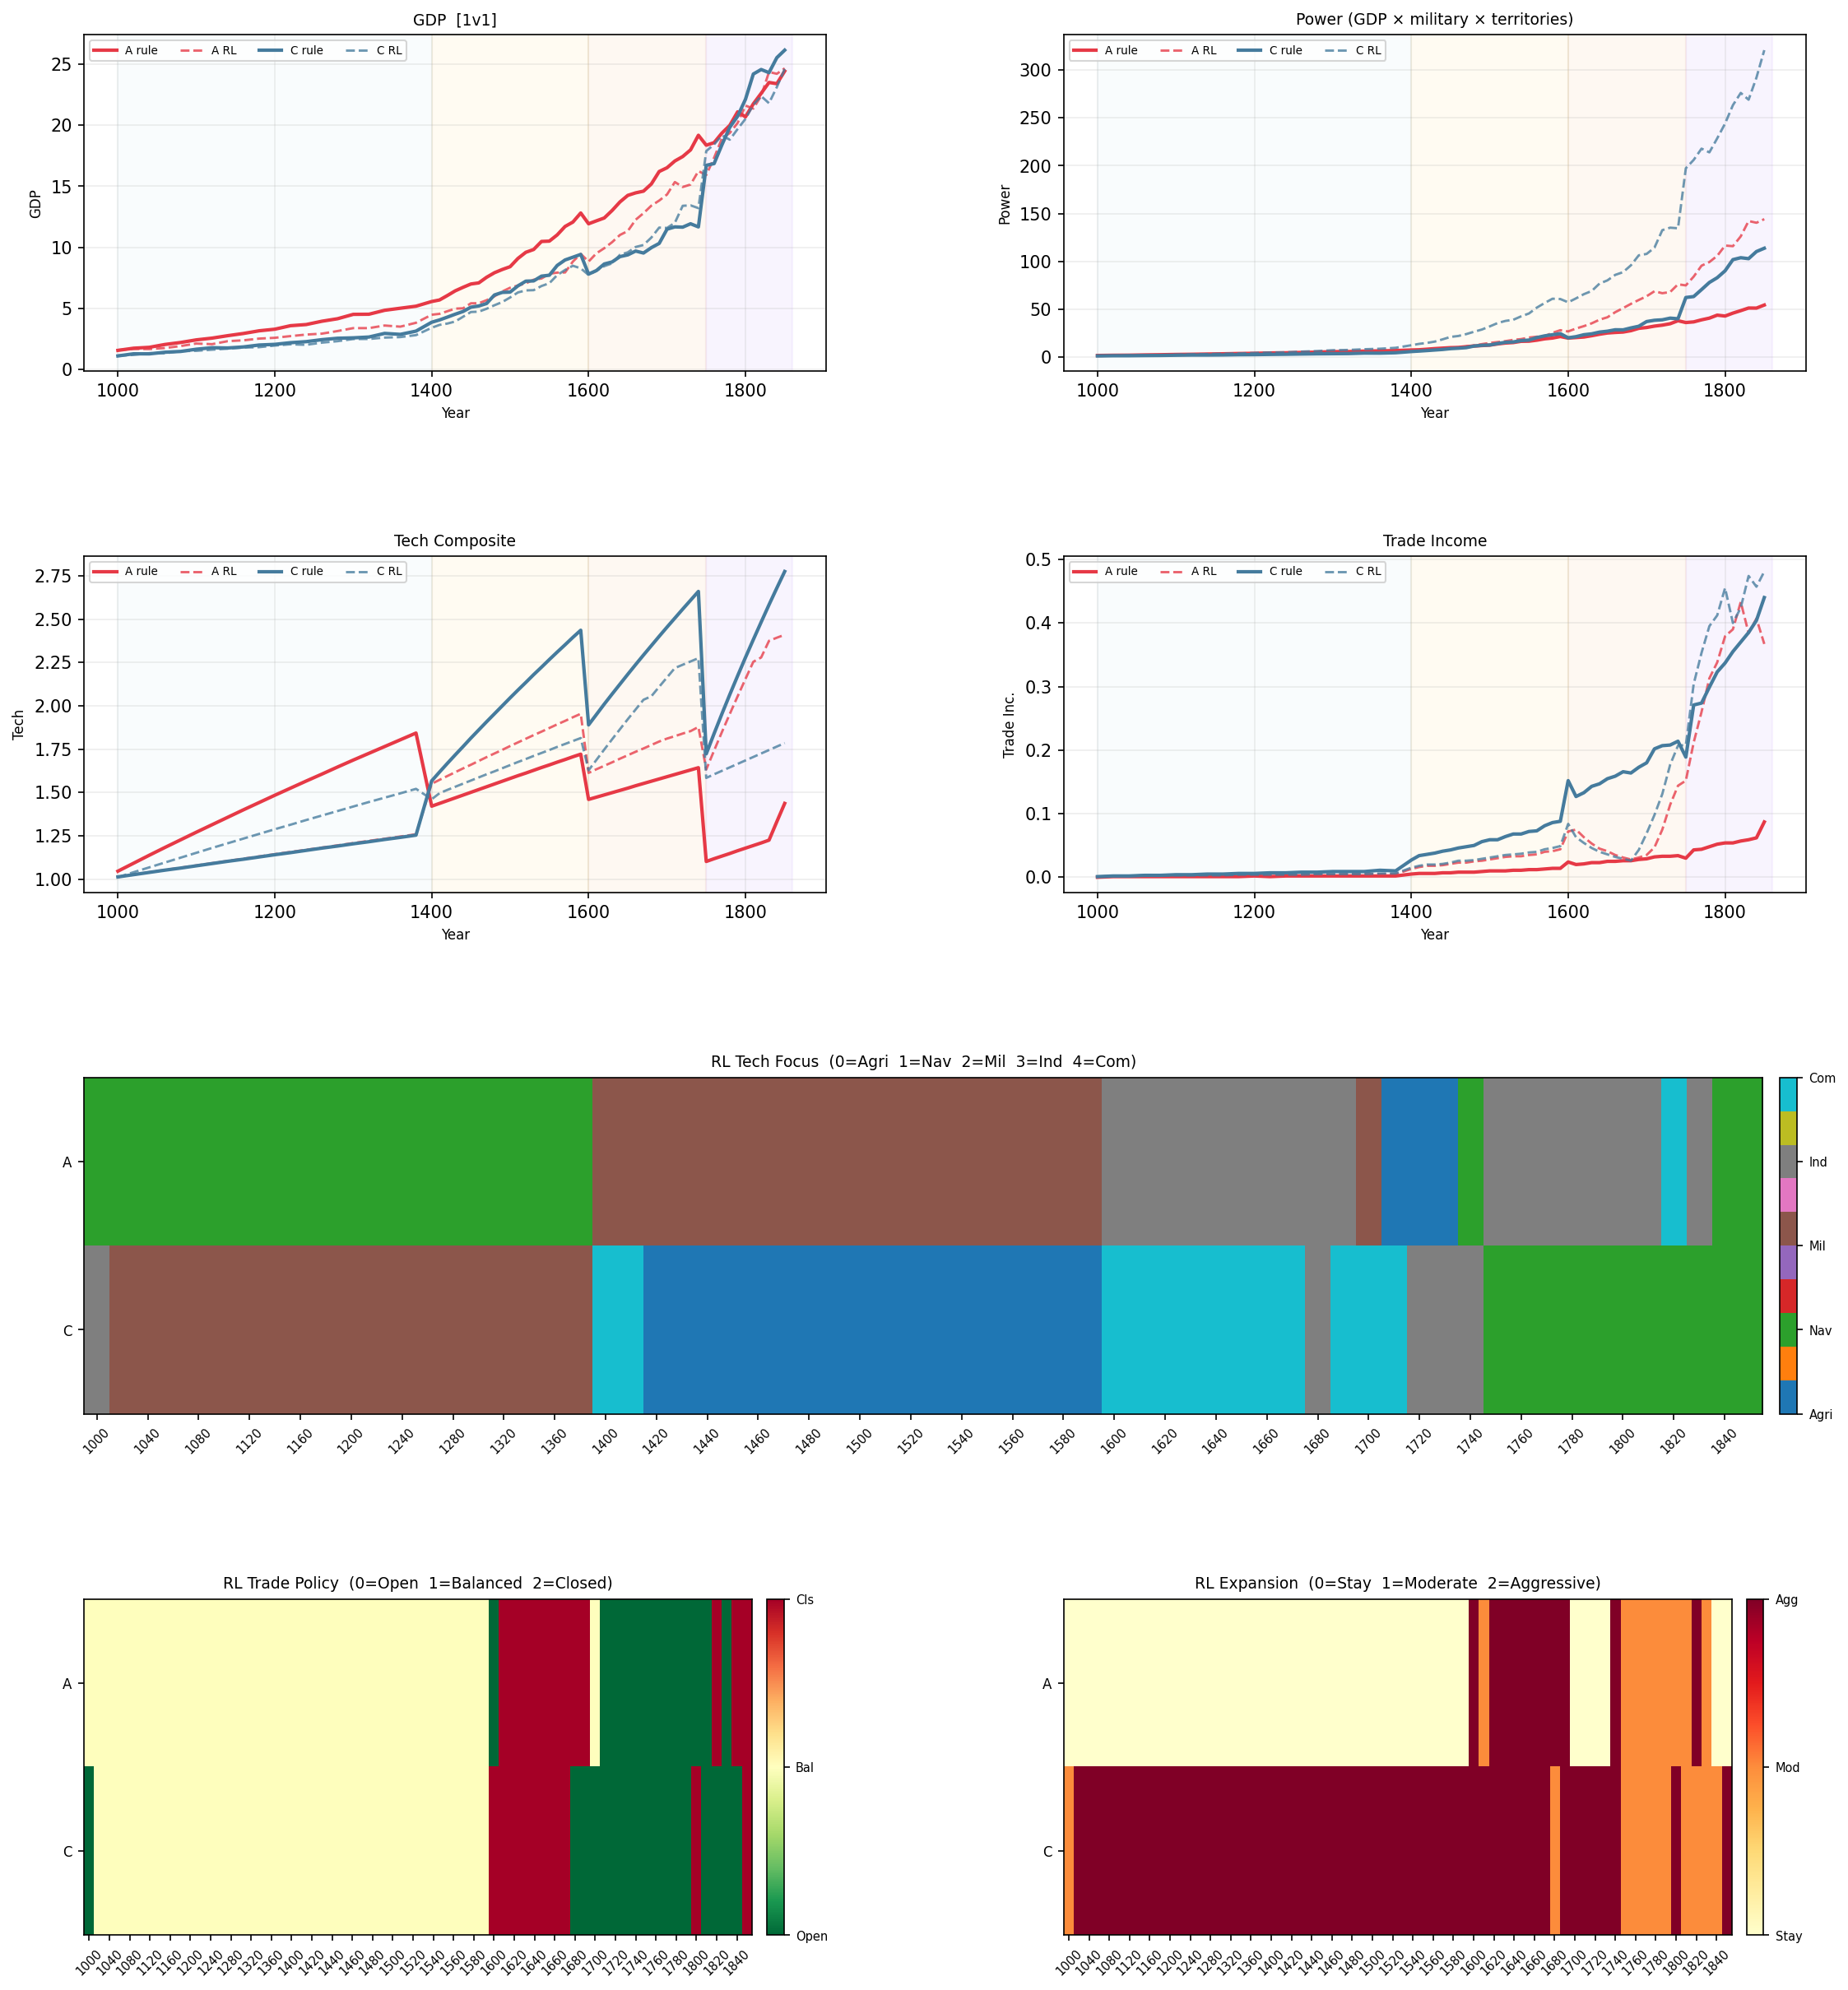
\includegraphics[width=0.80\textwidth]{with_coal.png}
    \caption{实验一：增加煤炭后农业文明 A 的工业化表现对比（含竞争激励）。}
    \label{fig:exp1}
\end{figure}

% ── 实验二 ──────────────────────────────────────────────────────
\subsection{实验二：东亚农业文明圈的粮食禀赋分化}

\textbf{实验设计：}构造五个初始地理与战略参数相近的农业文明，仅 A 文明的粮食禀赋明显高于其余四者（$R_{\text{food}}^A = 2.8$ vs. $R_{\text{food}}^{B\text{-}E} = 1.0$），均采用 RL 策略（综合国力目标）进行博弈。

\textbf{主要发现：}如图~\ref{fig:exp2} 所示，食物禀赋主导了人口增长（方程~\eqref{eq:carrying_capacity}），使 A 文明早期积累大量劳动力，GDP 及贸易收入均显著领先，演化为区域核心国。
值得注意的是，RL 优化后，\textbf{A 文明倾向于温和扩张与农业技术优先}以强化已有的劳动力优势；而食物禀赋较低的 B 文明在 RL 策略中转向\textbf{激进领土扩张与工业技术优先}，最终综合国力跃居区域第一，与日本明治维新后"以扩张代替禀赋不足"的历史路径高度吻合。

\begin{figure}[H]
    \centering
    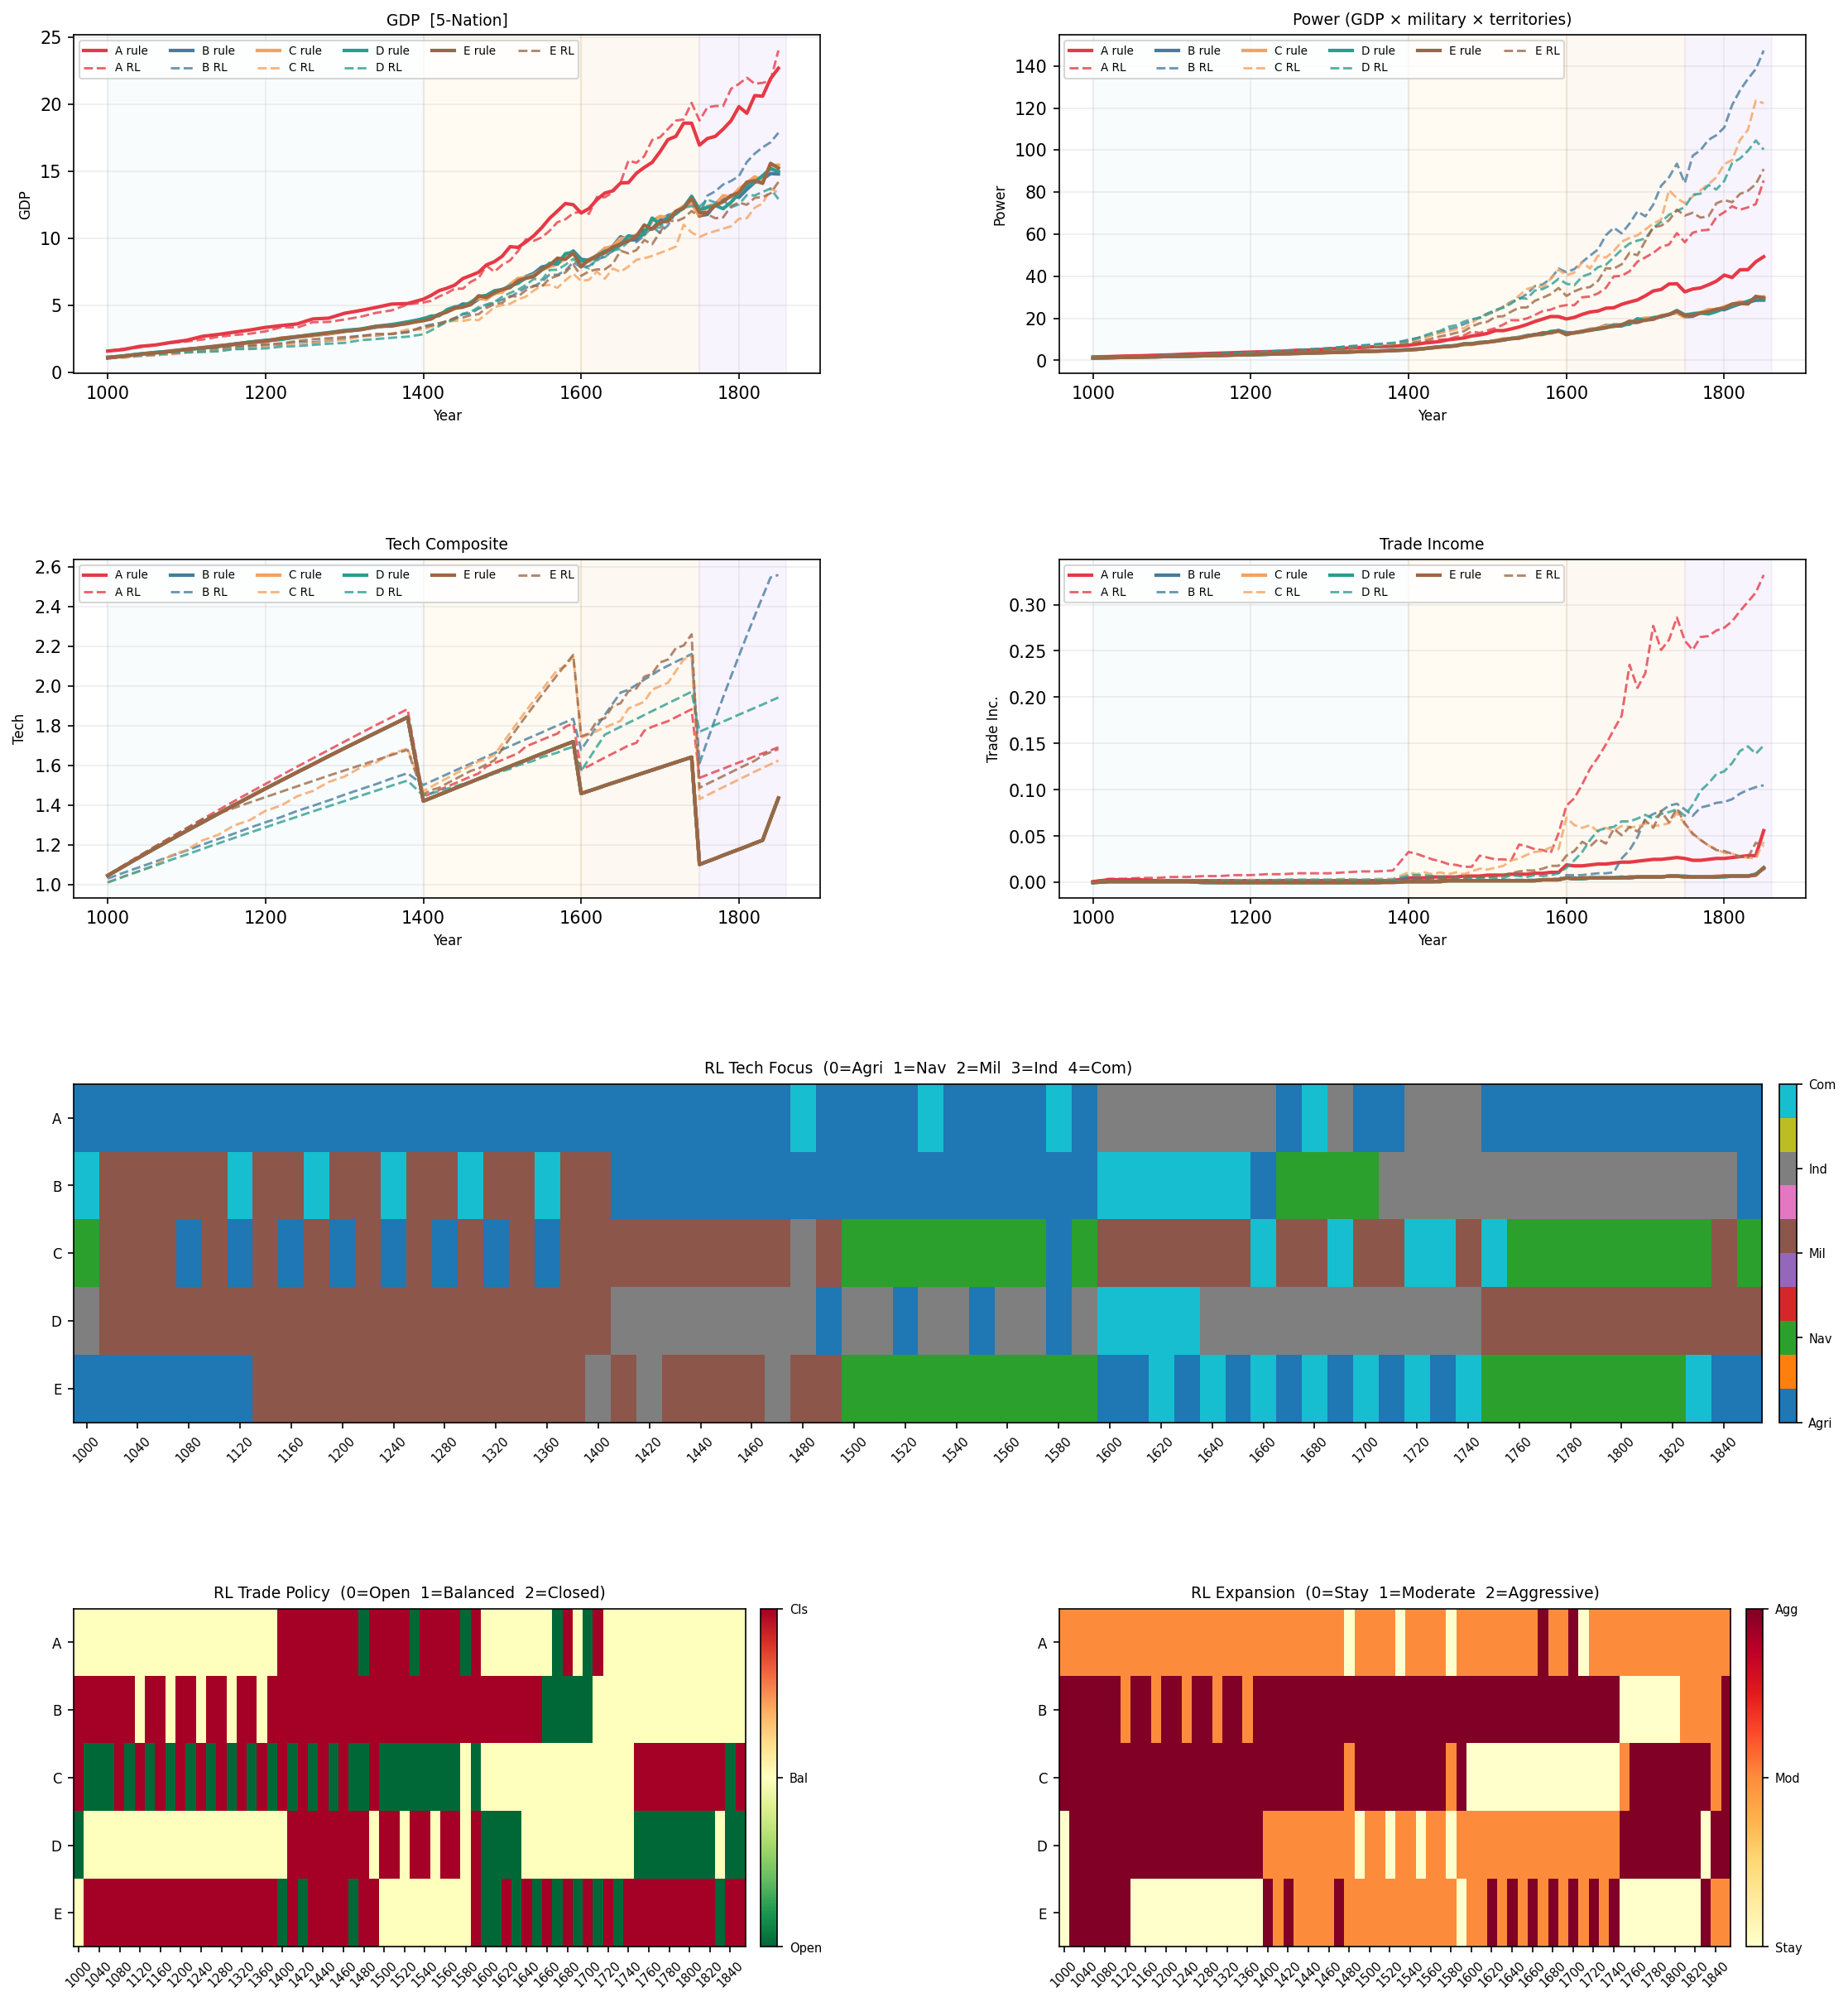
\includegraphics[width=0.80\textwidth]{rl_comparison_5_Nation.png}
    \caption{实验二：五文明农业圈 RL 对比（A 粮食禀赋 $=2.8$，B–E $=1.0$）。}
    \label{fig:exp2}
\end{figure}

% ── 实验三 ──────────────────────────────────────────────────────
\subsection{实验三：综合国力竞争激励对策略选择的影响}

\textbf{实验设计：}1v1 对局（A 农业 vs. C 工业），分别在\textbf{关闭}和\textbf{开启}竞争激励（方程~\eqref{eq:competitive}）条件下训练 RL 策略，对比策略偏好的变化。

\textbf{主要发现：}如图~\ref{fig:exp3} 所示，开启竞争激励后两文明均转向更激进的领土扩张，并在前工业化时期出现明显的\textbf{军备竞赛信号}（军事技术投入比例上升）。然而令人意外的是，两国贸易政策也同时转向\textbf{更高开放度}——贸易收入和殖民收入的双重提升抵消了军备开支，加速了双方的整体生产力增长。这为近代欧洲列强在军事竞争与贸易扩张\textit{并行}的背景下实现快速崛起提供了模型层面的解释，呼应了 North（1990）关于竞争性制度与经济增长关系的论述。

\begin{figure}[H]
    \centering
    \begin{subfigure}[b]{0.48\textwidth}
        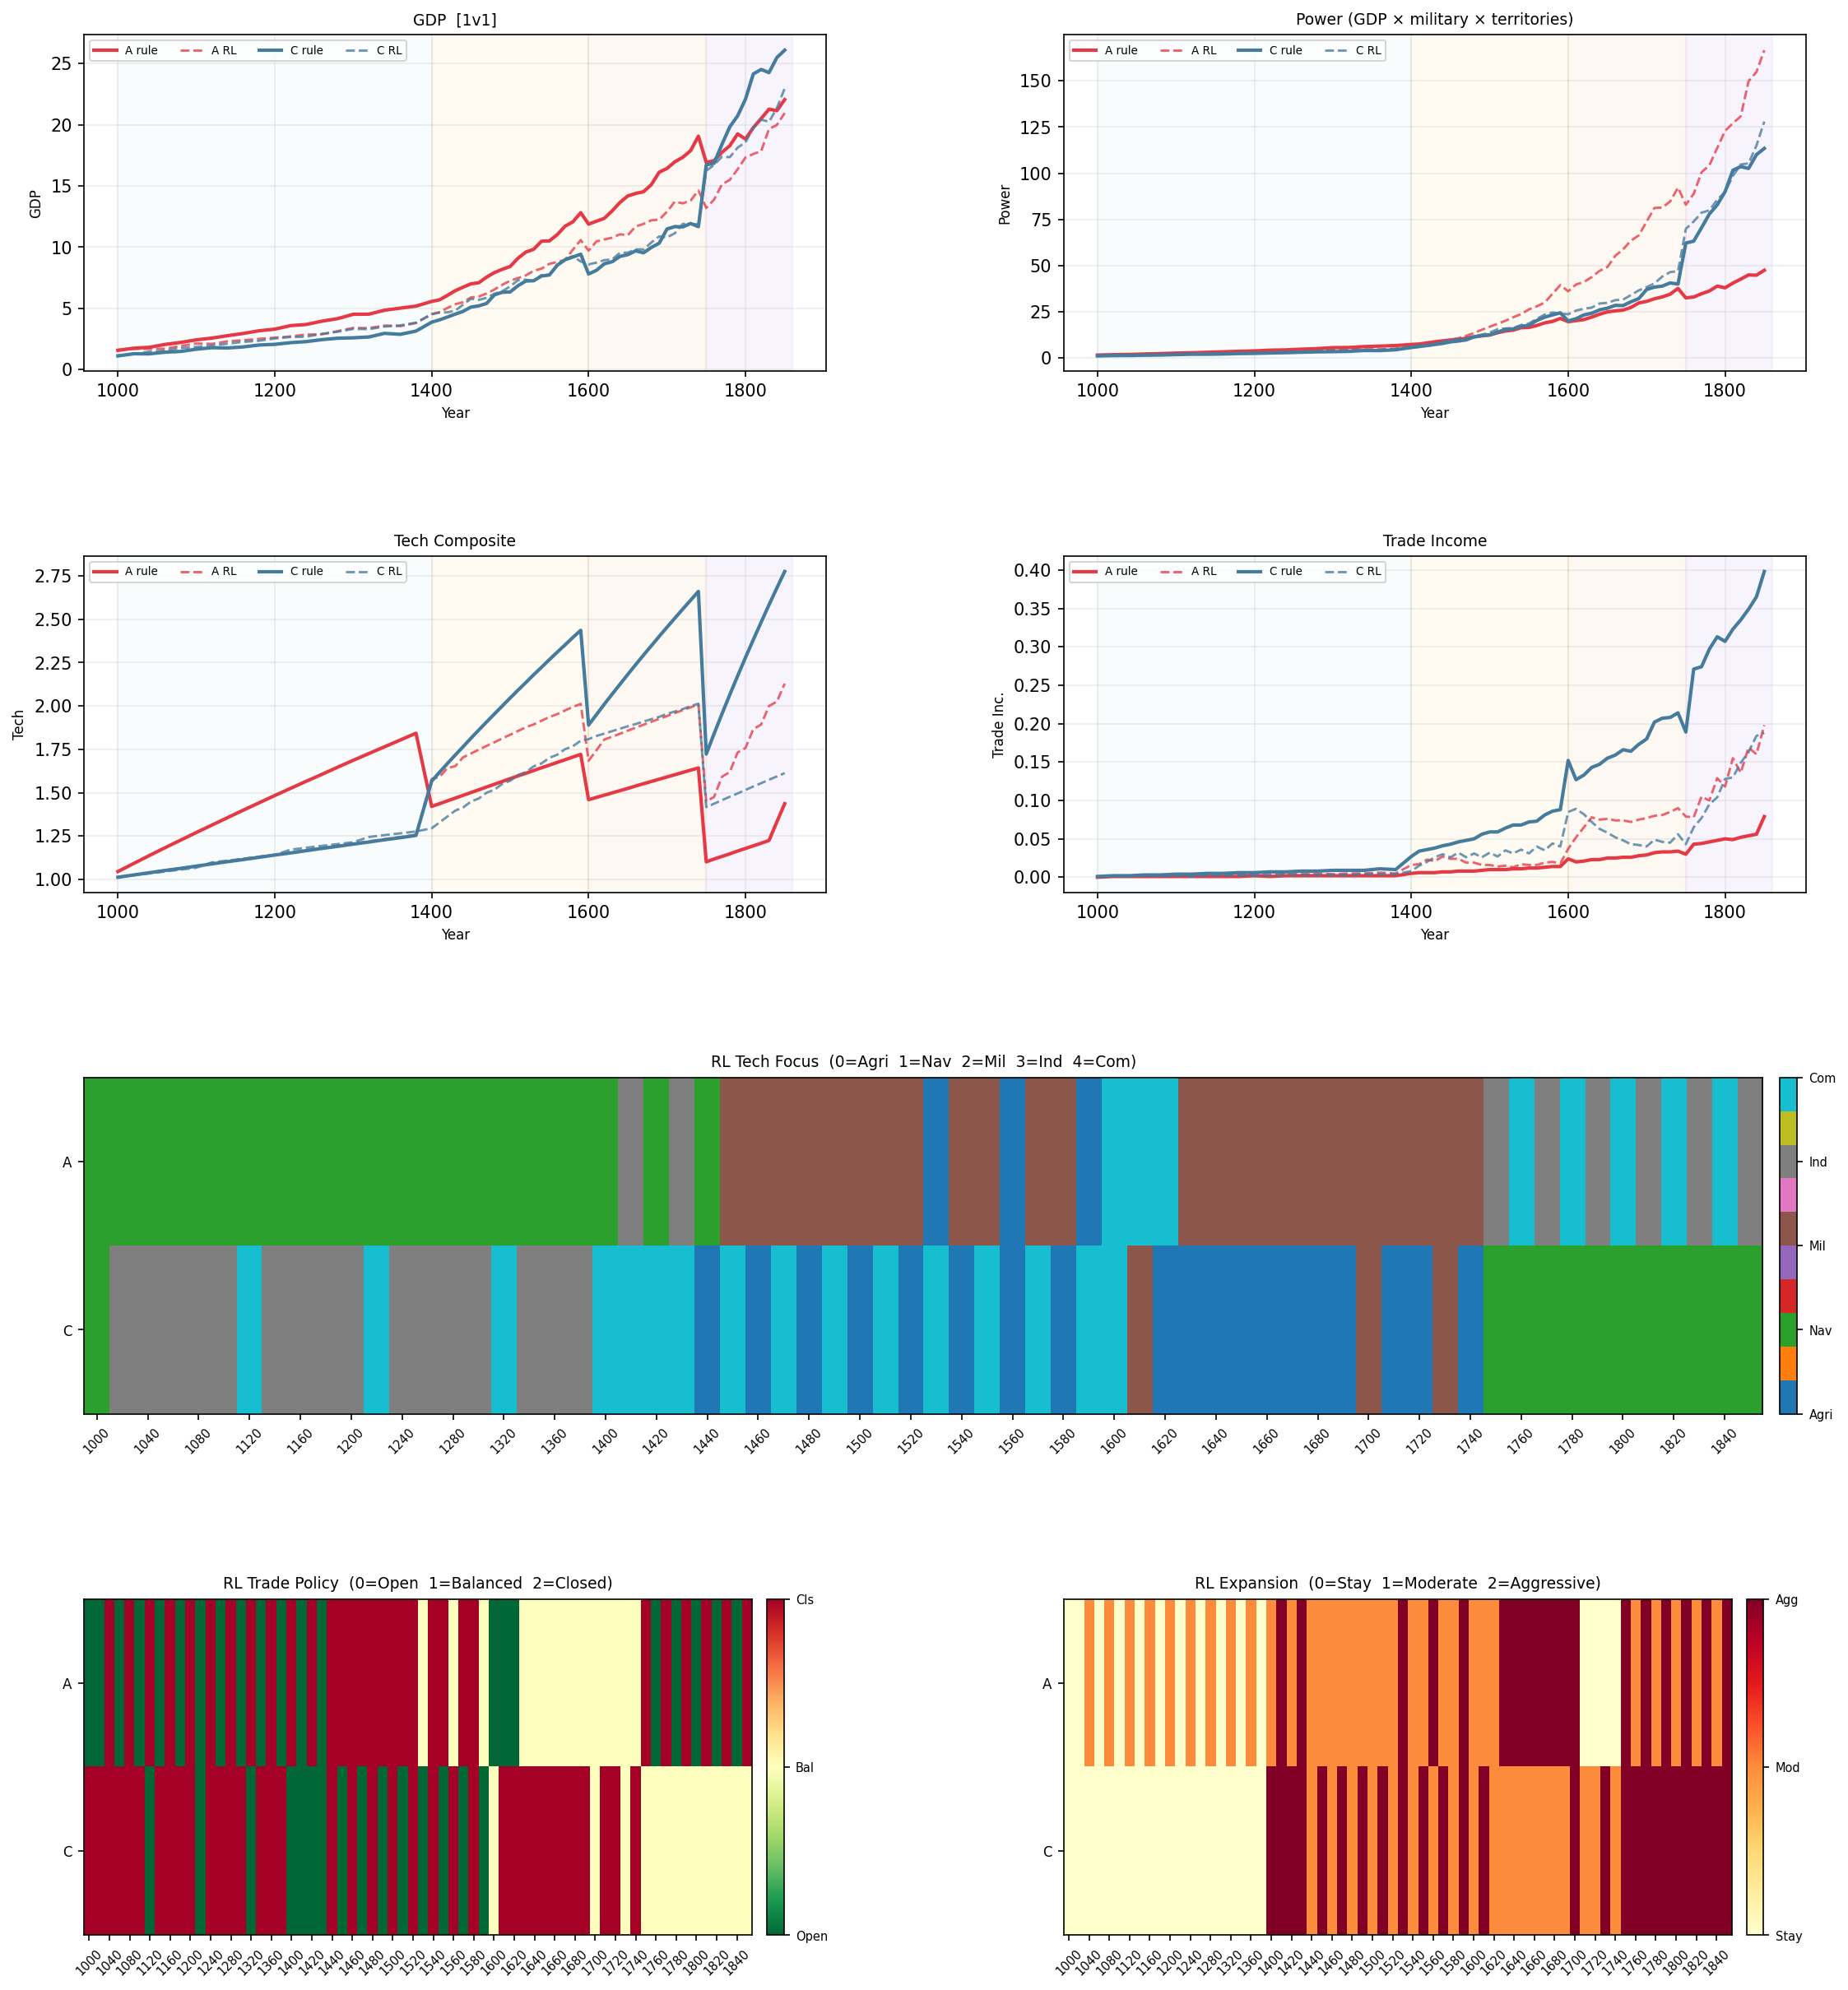
\includegraphics[width=\textwidth]{1v1_no_compe.png}
        \caption{关闭竞争激励}
    \end{subfigure}
    \hfill
    \begin{subfigure}[b]{0.48\textwidth}
        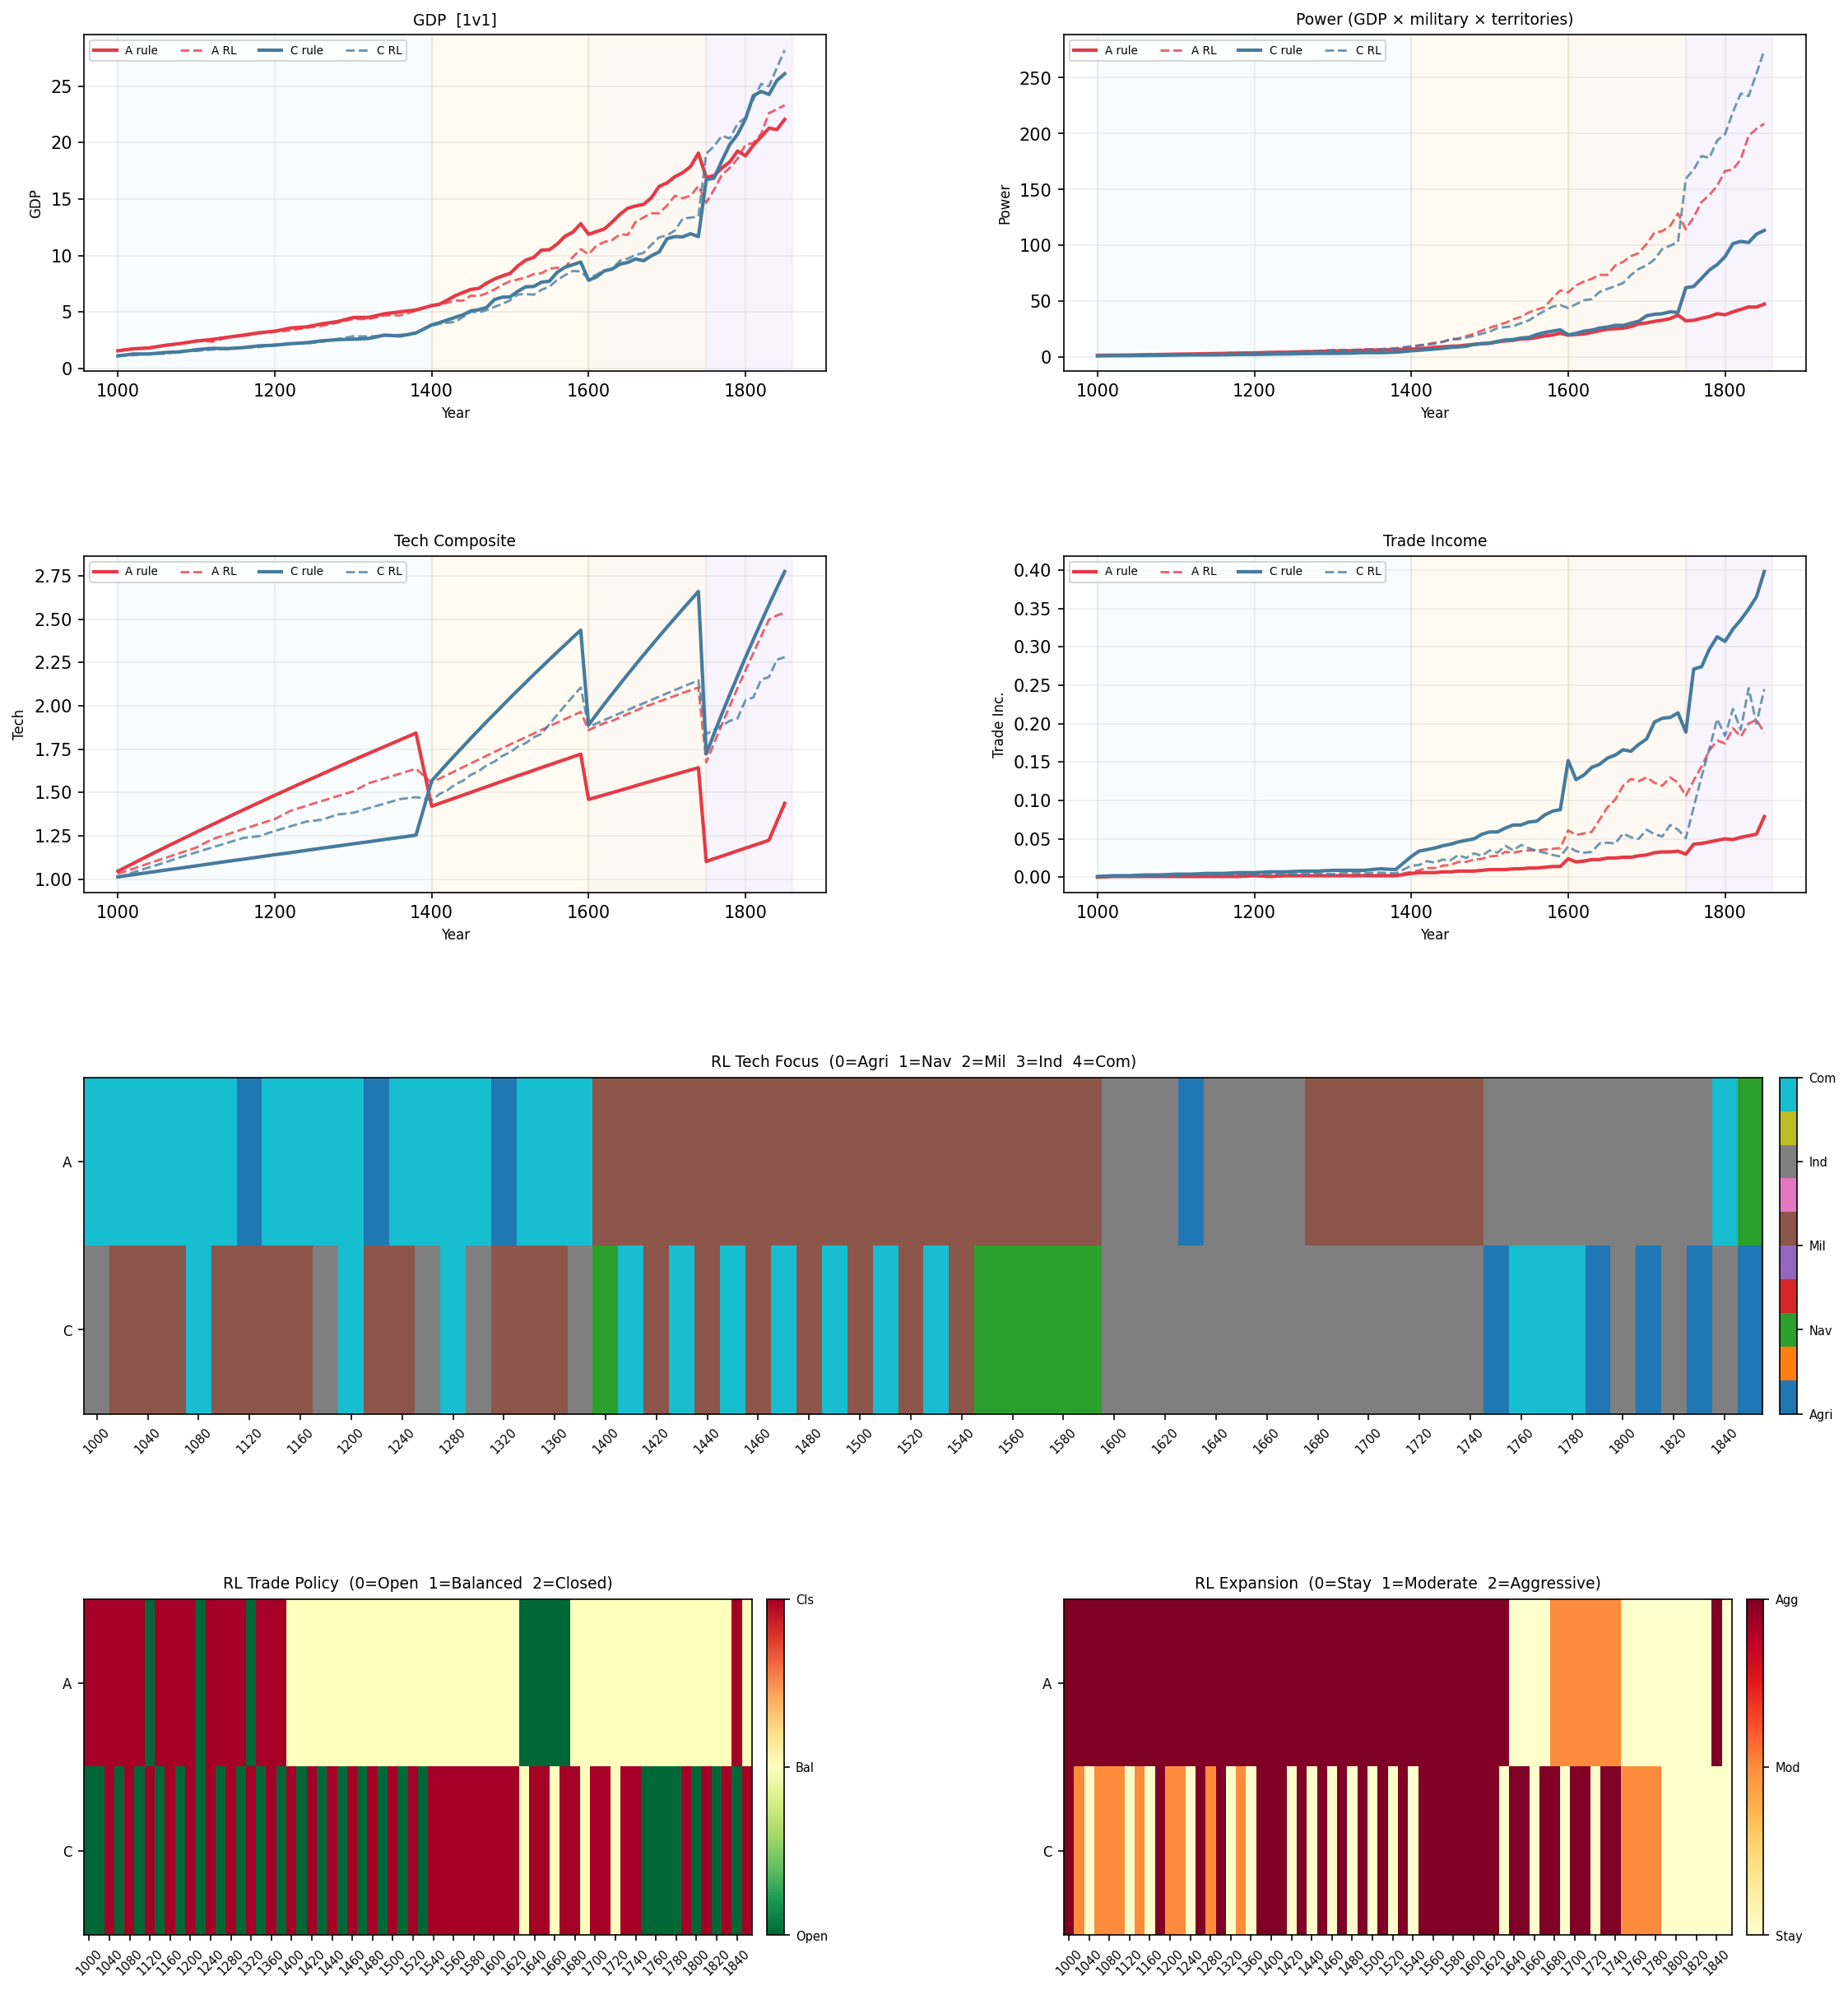
\includegraphics[width=\textwidth]{1v1_compe.png}
        \caption{开启竞争激励（$w_c=0.25$）}
    \end{subfigure}
    \caption{实验三：竞争激励对 RL 策略选择的影响（A 农业 vs. C 工业）。}
    \label{fig:exp3}
\end{figure}

% ── 实验四 ──────────────────────────────────────────────────────
\subsection{实验四：策略替换反事实——农业禀赋能否支撑工业化策略？}

\textbf{实验设计：}保持文明 A 的地理与资源禀赋不变，将其策略由 \textit{AgrarianConservative} 替换为 \textit{IndustrialPioneer}，与标准工业文明 C 进行 1v1 对比。通过规则策略排除 RL 随机性，聚焦战略选择的纯效应。

\textbf{主要发现：}如图~\ref{fig:exp4} 所示，策略替换使 A 文明终局 GDP 由 22.05 提升至 23.90（$+8.4\%$），技术综合指数由 1.44 跃升至 2.77（与 C 持平）。然而，人均 GDP 仅从 0.150 提升至 0.224，而 C 文明的人均 GDP 达到 0.433，差距依然悬殊。关键机制在于：A 文明庞大的人口（高粮食承载上限）在工业化路径下\textbf{成为负担而非优势}——人均资本积累速度受制于 $L^\alpha$ 项中的人口摊薄效应（方程~\eqref{eq:cobb_douglas}）。这一结果复现了"高水平均衡陷阱"（High-Level Equilibrium Trap，Elvin 1973）的核心机制：庞大的人口基数使农业文明即便改变战略，也难以在人均生产力上追赶煤炭资源丰富的工业国。

\begin{figure}[H]
    \centering
    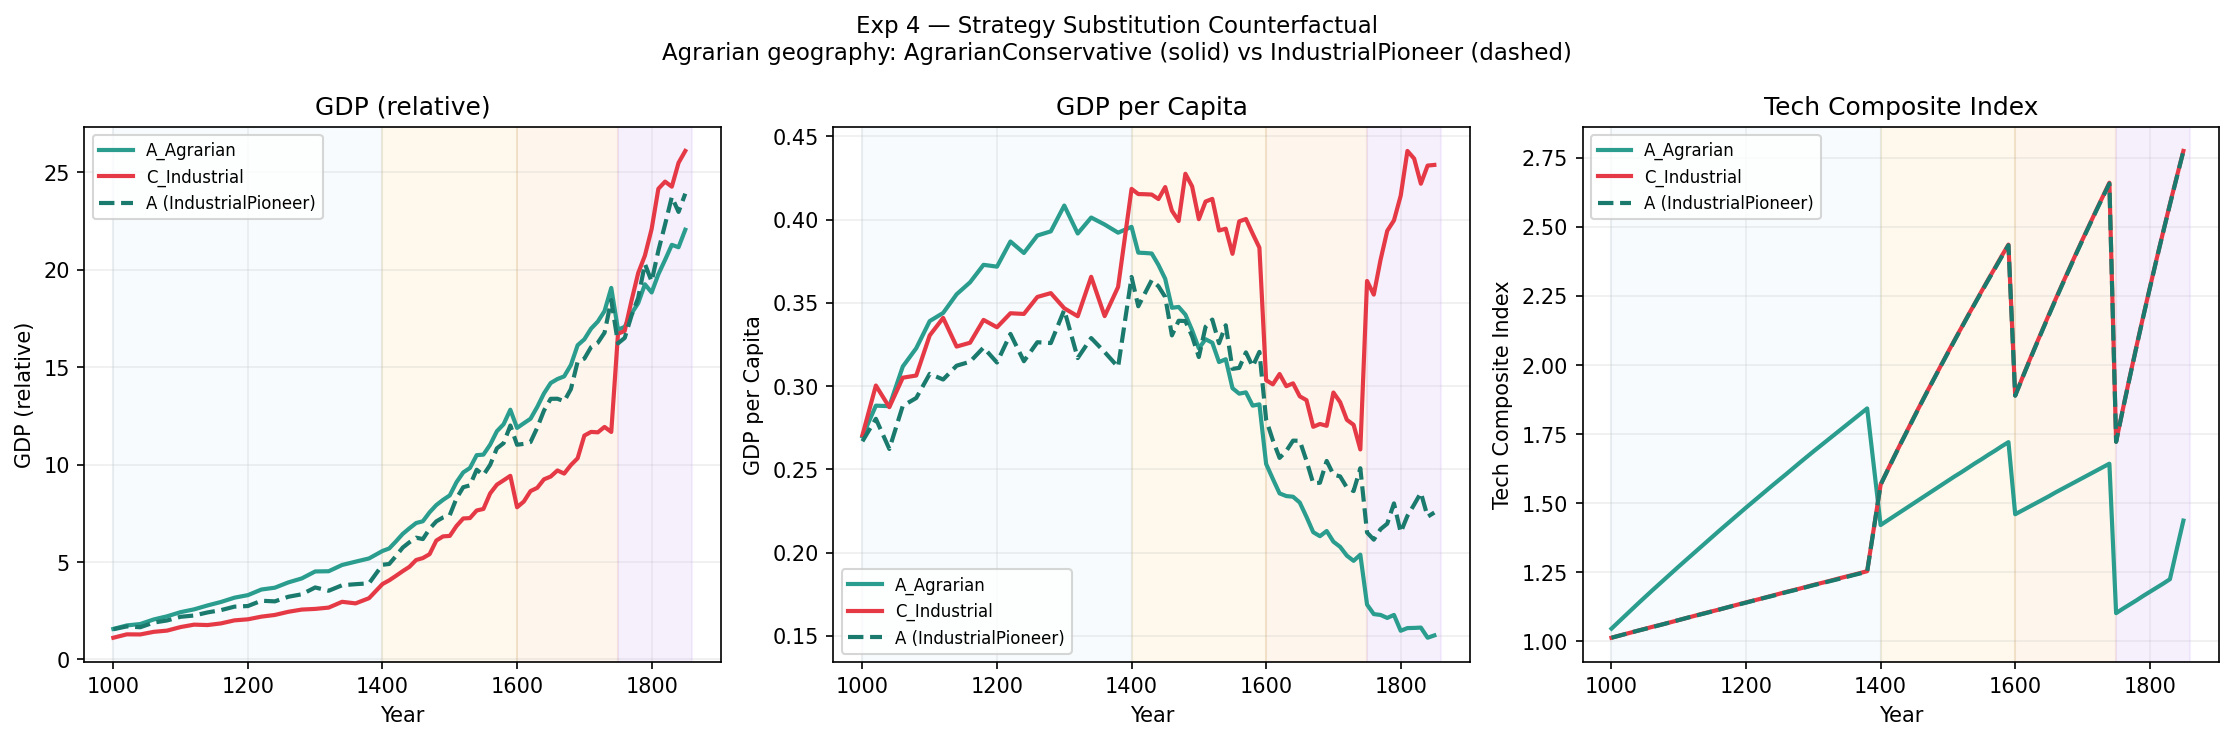
\includegraphics[width=\textwidth]{exp4_strategy_substitution.png}
    \caption{实验四：策略替换反事实（A 保持原始禀赋，比较三种历史路径）。虚线为 A 改采工业先驱策略。}
    \label{fig:exp4}
\end{figure}

\begin{table}[H]
\centering
\caption{实验四终局指标对比（1850年）}
\label{tab:exp4}
\begin{tabular}{lccc}
\toprule
情景 & 终局 GDP & 人均 GDP & 技术综合指数 \\
\midrule
A（农业保守策略）     & 22.05 & 0.150 & 1.44 \\
A（工业先驱策略替换） & 23.90 & 0.224 & 2.77 \\
C（工业先驱策略）     & 26.10 & 0.433 & 2.77 \\
\bottomrule
\end{tabular}
\end{table}

% ── 实验五 ──────────────────────────────────────────────────────
\subsection{实验五：五强全规则策略的长期自然均衡}

\textbf{实验设计：}五种文明原型（A–E）均采用对应历史原型的规则策略，在 5-Nation 竞争模式下运行完整历史时间轴，形成无 RL 干扰的"历史惯性"基准均衡。

\textbf{主要发现：}如图~\ref{fig:exp5} 及表~\ref{tab:exp5} 所示，终局 GDP 排名为 C$>$E$>$A$>$D$>$B，但人均 GDP 排名倒置为 C$>$D$>$E$>$B$>$A，揭示出三条关键规律：

\begin{enumerate}
    \item \textbf{总量 vs. 人均的分离}：农业大国 A 总 GDP 居中但人均 GDP 垫底（0.157），呈现典型 Malthusian 陷阱——高承载人口压低人均资本。
    \item \textbf{贸易枢纽的专业化优势}：D（高战略位置）贸易收入最高（1.987），技术综合指数领先（2.945），靠商业技术积累实现高人均 GDP（0.412），但总量受限于不扩张策略。
    \item \textbf{工业化的迟到溢价}：C 直到工业时代才开始拉开与 E 的差距，前三个时代的规则策略差异有限，工业革命的煤炭 TFP 红利（$\Delta A \approx 0.22$）是最终分化的主要驱动。
\end{enumerate}

\begin{figure}[H]
    \centering
    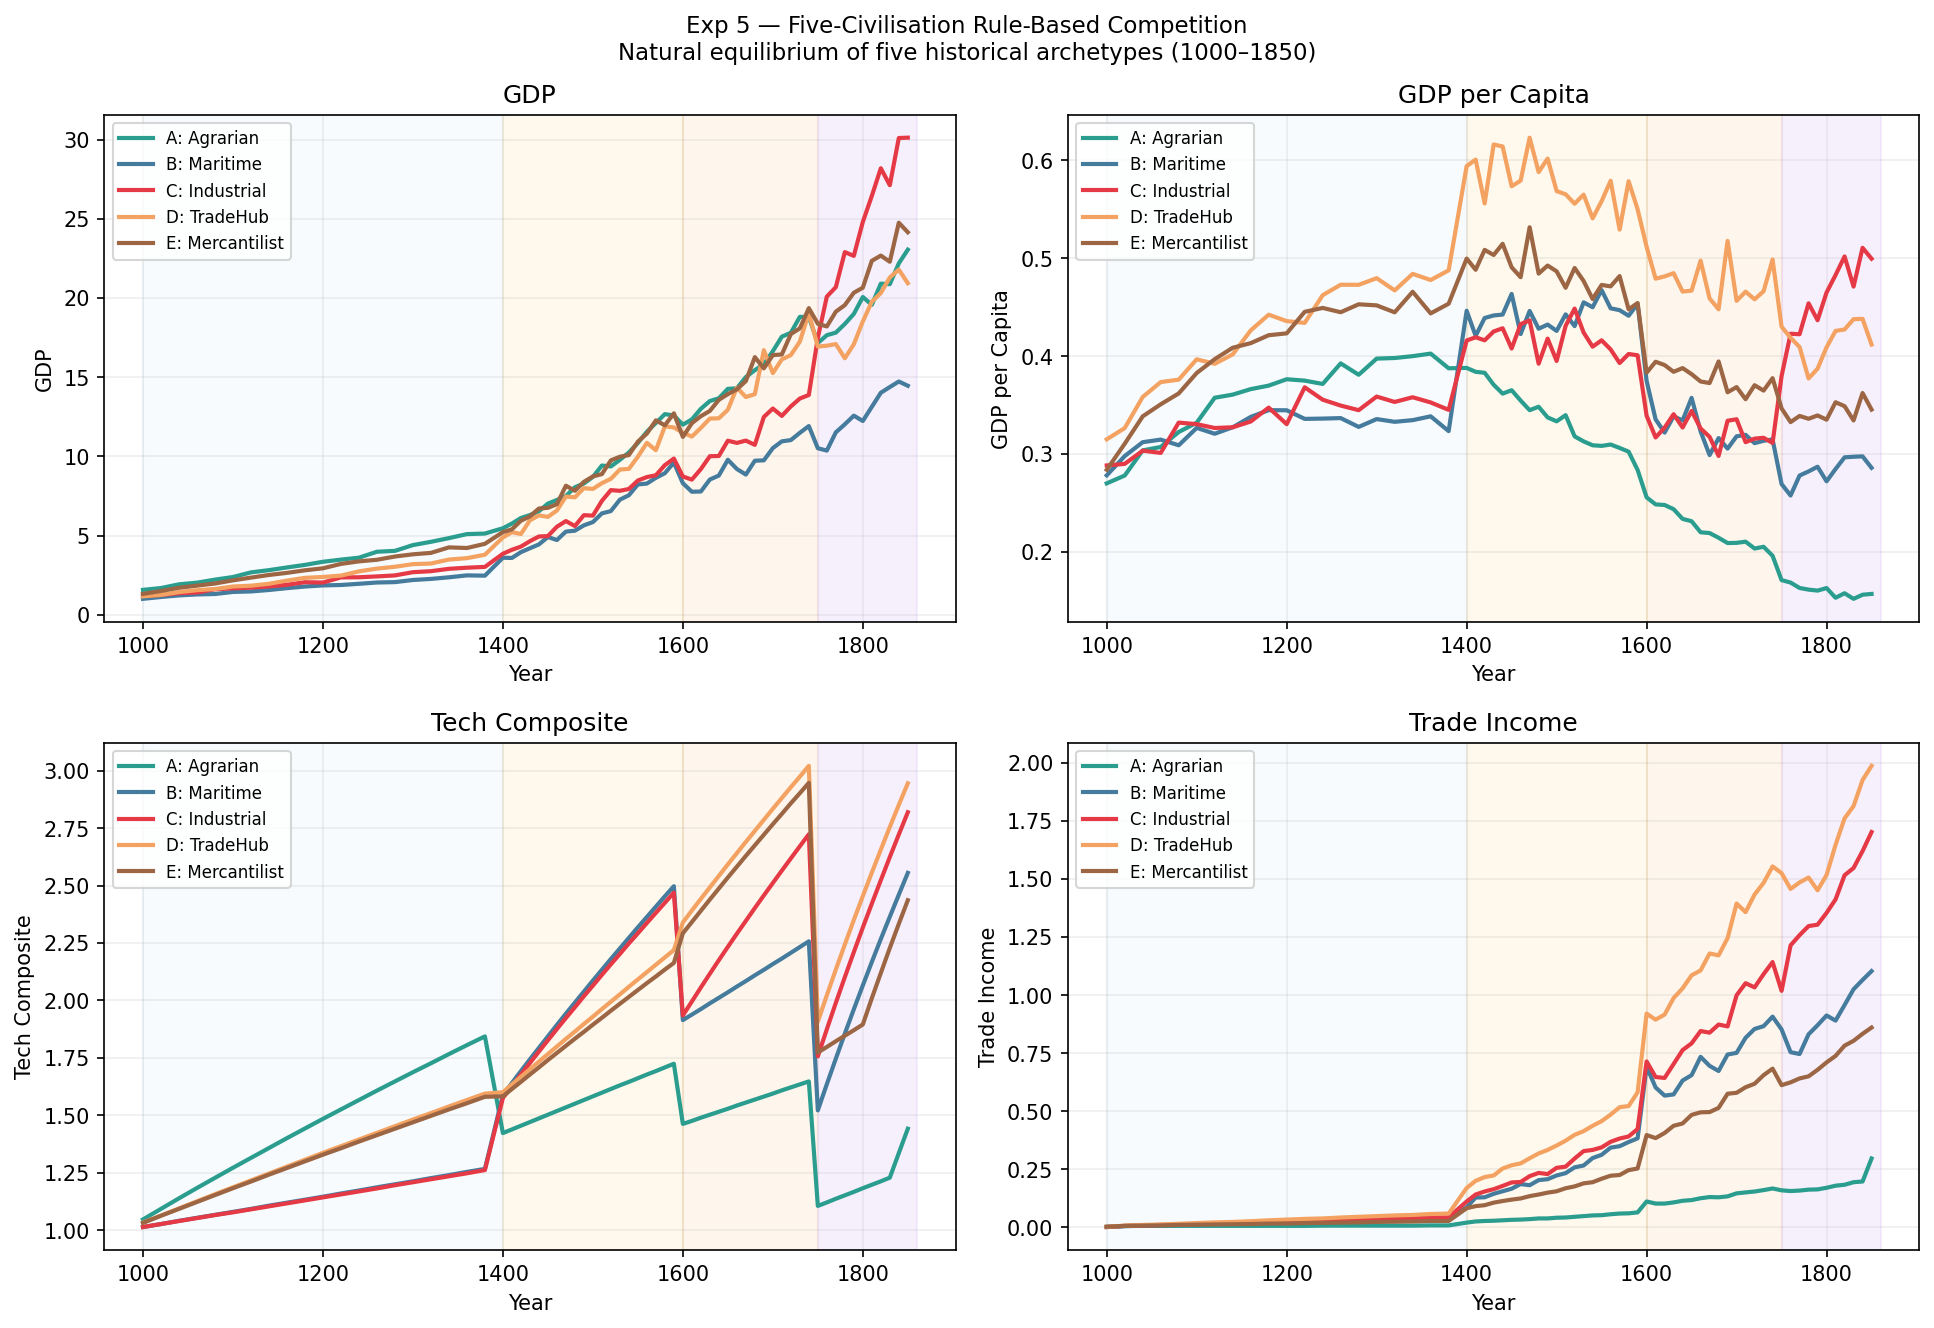
\includegraphics[width=\textwidth]{exp5_five_nation_rule.png}
    \caption{实验五：五强全规则策略的历史均衡轨迹（1000–1850年，四面板）。}
    \label{fig:exp5}
\end{figure}

\begin{table}[H]
\centering
\caption{实验五终局指标（1850年，规则策略）}
\label{tab:exp5}
\begin{tabular}{lcccc}
\toprule
文明 & GDP & 人均 GDP & 技术指数 & 贸易收入 \\
\midrule
C（工业先驱） & 30.12 & 0.500 & 2.819 & 1.702 \\
E（重商主义） & 24.15 & 0.345 & 2.436 & 0.860 \\
A（农业保守） & 23.04 & 0.157 & 1.441 & 0.296 \\
D（贸易枢纽） & 20.93 & 0.412 & 2.945 & 1.987 \\
B（航海扩张） & 14.45 & 0.286 & 2.555 & 1.103 \\
\bottomrule
\end{tabular}
\end{table}

% ── 实验六 ──────────────────────────────────────────────────────
\subsection{实验六：三国 RL 博弈中的策略涌现与均衡陷阱}

\textbf{实验设计：}3-Nation 模式（A/B/C），三方均使用综合国力最大化（Power）RL 策略并开启竞争激励，训练 120 个 episode，对比规则策略基准。

\textbf{主要发现：}如图~\ref{fig:exp6} 及表~\ref{tab:exp6} 所示，竞争 RL 相对规则策略\textbf{所有三方 GDP 均下降}（A: $-10\%$，B: $-10\%$，C: $-13\%$），形成典型的多方竞争困境。技术偏好热力图进一步揭示了策略分化：A 在前期（中世纪/大发现）集中农业技术，工业时代切换至工业/商业，反映出 RL 对初始禀赋的自适应；B 大量探索了导航与商业技术组合；C 则自始坚持工业技术投入。

这一结果与博弈论的预言一致：\textbf{纯国力竞争的 Nash 均衡是集体次优的}——所有文明将资源导向相互抵消的军备扩张，而非互补性的分工贸易，最终导致整体福利低于合作均衡。历史上，多极化时代（如19世纪欧洲均势体系与20世纪初军备竞赛）的重复军备耗损与此机制吻合。

\begin{figure}[H]
    \centering
    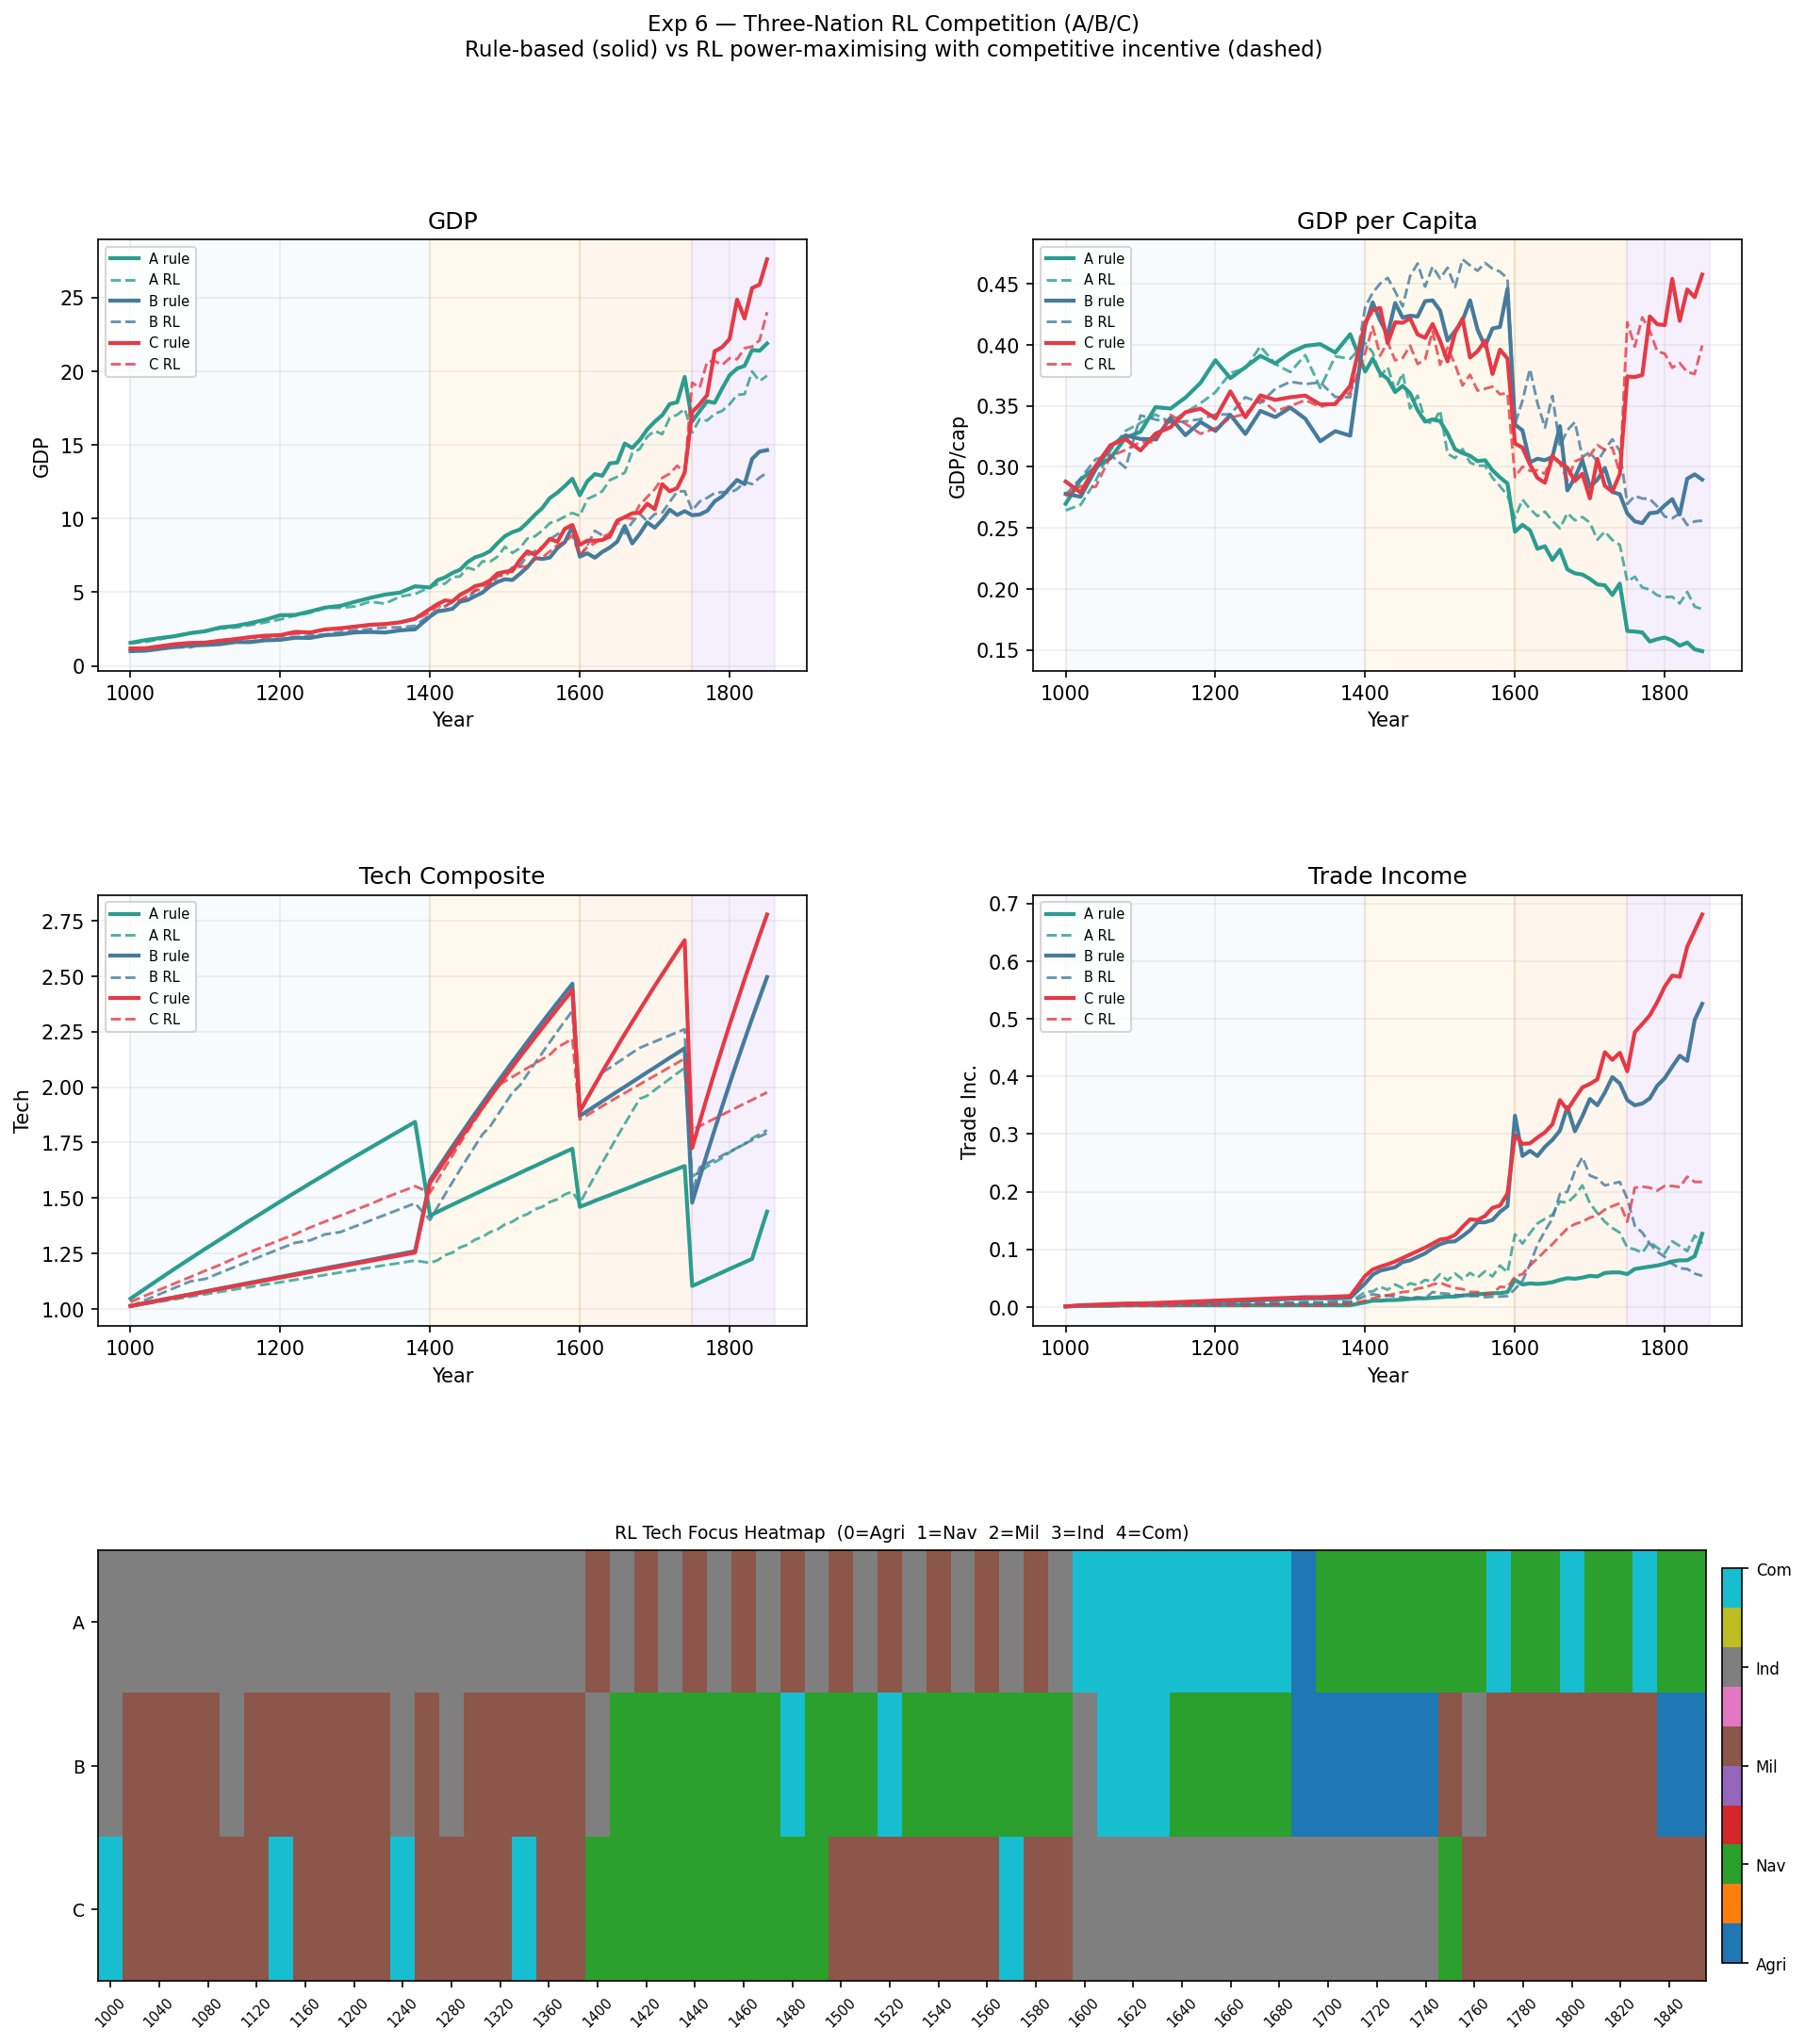
\includegraphics[width=\textwidth]{exp6_three_nation_rl.png}
    \caption{实验六：三国竞争 RL 策略（实线=规则，虚线=RL）。下方热力图为 RL 技术偏好随时间演变。}
    \label{fig:exp6}
\end{figure}

\begin{table}[H]
\centering
\caption{实验六终局 GDP 对比（规则策略 vs. 竞争 RL，1850年）}
\label{tab:exp6}
\begin{tabular}{lrrrr}
\toprule
文明 & 规则策略 GDP & RL 策略 GDP & 绝对差 & 相对差 \\
\midrule
A（农业保守） & 21.88 & 19.69 & $-2.19$ & $-10.0\%$ \\
B（航海扩张） & 14.64 & 13.10 & $-1.54$ & $-10.5\%$ \\
C（工业先驱） & 27.59 & 24.00 & $-3.59$ & $-13.0\%$ \\
\bottomrule
\end{tabular}
\end{table}

\paragraph{跨实验综合解读} 六组实验共同指向三个层次的结论：（1）\textbf{地理决定论的局限性}——煤炭（实验一）和海岸条件的联合作用远强于单一资源改变，但策略替换（实验四）仍能带来有限但真实的追赶效果；（2）\textbf{历史策略原型的路径依赖}——规则策略基准（实验五）下，各文明禀赋与策略形成的惯性路径基本复现了1000–1850年间的经济分化格局；（3）\textbf{竞争的双重面孔}——1v1 竞争激励（实验三）促进双方开放贸易与生产力增长，而三方竞争 RL（实验六）则形成囚徒困境式的集体损耗，提示竞争格局的极性（双极 vs. 多极）可能对均衡结果产生根本性影响。

% ──────────────────────────────────────────────────────────────────
\section{局限性与后续方向}
% ──────────────────────────────────────────────────────────────────

本模型在以下方面存在简化：其一，生产函数忽略劳动参与率与土地的独立角色，资本弹性标定未作正式校准；其二，贸易收益函数假设比较优势持续存在，未建模技术引进带来的禀赋结构改变；其三，Q-learning 的状态离散化导致大量状态聚合，可能掩盖边界效应。后续可引入深度 Q 网络（DQN）以处理连续状态空间，并结合历史面板数据对 TFP 参数进行矩估计校准，提升模型的实证基础。

% ──────────────────────────────────────────────────────────────────
\begin{thebibliography}{9}
\bibitem{pomeranz2000} Pomeranz, K. (2000). \textit{The Great Divergence: China, Europe, and the Making of the Modern World Economy}. Princeton University Press.

\bibitem{acemoglu2001} Acemoglu, D., Johnson, S., \& Robinson, J. A. (2001). The colonial origins of comparative development: An empirical investigation. \textit{American Economic Review}, 91(5), 1369--1401.

\bibitem{solow1956} Solow, R. M. (1956). A contribution to the theory of economic growth. \textit{Quarterly Journal of Economics}, 70(1), 65--94.

\bibitem{hasselt2010} Hasselt, H. V. (2010). Double Q-learning. \textit{Advances in Neural Information Processing Systems}, 23, 2613--2621.

\bibitem{diamond1997} Diamond, J. (1997). \textit{Guns, Germs, and Steel: The Fates of Human Societies}. W.W. Norton.

\bibitem{north1990} North, D. C. (1990). \textit{Institutions, Institutional Change and Economic Performance}. Cambridge University Press.

\bibitem{elvin1973} Elvin, M. (1973). \textit{The Pattern of the Chinese Past}. Stanford University Press.

\bibitem{wrigley1988} Wrigley, E. A. (1988). \textit{Continuity, Chance and Change: The Character of the Industrial Revolution in England}. Cambridge University Press.
\end{thebibliography}

\end{document}
